\documentclass[siggraph]{acmart}

\setcopyright{none}
\settopmatter{printacmref=false} % Removes citation information below abstract
\renewcommand\footnotetextcopyrightpermission[1]{} % removes footnote with conference information in first column
\pagestyle{plain}

\usepackage{booktabs} % For formal tables
\usepackage{listings}
\usepackage{courier}

\lstset{basicstyle=\footnotesize\ttfamily,breaklines=true}

\begin{document}
\title{Occlusion in outdoor Augmented Reality using geospatial building data}
\titlenote{Master Degree Project in Computer Science and Communication.}

\author{Johan Kasperi}
\affiliation{
  \institution{KTH Royal Institute of Technology}
  \city{Stockholm}
  \country{Sweden}
}
\email{kasperi@kth.se}

\begin{abstract}
Creating physical simulations between virtual and real objects in \textit{Augmented Reality} (AR) is essential for the user experience. Otherwise the user might lose sense of depth, distance and size. One of these simulations is occlusion, meaning that virtual content should be partially or fully occluded if real world objects is in the line-of-sight between the user and the content. The challenge for simulating occlusion is to construct the geometric model of the current AR environment. Earlier studies within the field have all tried to create realistic pixel-perfect occlusion and most of them have either required special depth-sensing hardware or a static predefined environment. This study proposes and evaluates an alternative model-based approach to the problem. It uses geospatial data to construct the geometric model of all the buildings in the current environment, making virtual content occluded by all real buildings in the current environment. This approach made the developed function compatible on non depth-sensing devices and in a dynamic outdoor urban environment. To evaluate the solution it was implemented in an sensor-based AR application visualizing a future building in Stockholm. The effect of the developed function was that the future virtual building was occluded as expected. However, it was not pixel-perfect, meaning that the simulated occlusion was not realistic, but results from the conducted user study said that it fulfilled its goal. A majority of the participants thought that their AR experience got better with the solution activated and that their depth perception improved. But any definite conclusions could not be drawn due to issues with the sensor-based tracking. The result is interesting for the mobile AR field since the great majority of smartphones are not equipped with depth sensors. Using geospatial data for simulating occlusions, or other physical interactions between the virtual and real objects, could then be an efficient enough solution until depth-sensing AR devices get more widely used.
\end{abstract}

\keywords{Augmented Reality, AR, Occlusion, Physical simulation, Geospatial data, Open Street Maps}

\maketitle

\section{Introduction}
\textit{Augmented Reality} (AR), is the medium that supplements the reality with virtual content such as sound, video, images or 3D objects \cite{azuma1997survey} by attaching content to a physical location, creating the effect of a virtual layer on top of the reality. The true strength of AR is that the users are enabled to see an enhanced reality with content that they ordinarily cannot see, for example making the construction worker see the beams inside a wall before they put their drill in it or the home decorator see the real size of a sofa before buying it \cite{venturebeatWalls, newatlasIkea}. The technology has the potential of providing us with information about the real world in real time as we see it. This invites to interesting usage areas in fields such as construction, education and gaming among others. 
The term \textit{Augmented Reality} was first coined in 1992 \cite{caudell1992augmented} but the first AR system was made back in 1965 \cite{sutherland1968head}. Early AR systems required expensive hardware and a lot of custom development efforts, making them only available for governments and companies \cite{azuma2016most}. But the recent years of development in AR hardware, software and applications, as well as its sister technology \textit{Virtual Reality} (VR), has made the technology relevant for everybody. Especially since the first release of the smartphone and its rapid development during the last decade. The smartphone made AR accessible for everyone and AR applications has already reached the consumers, for example the summer 2016 success game Pok\'emon GO \cite{azuma2016most}. The smartphone has pushed the development of so called \textit{Mobile AR Systems} (MARS), which are AR systems developed for usage out in the real world and far away from the research labs \cite{hollerer2004mobile}. However, the field still has some problems until it fulfills its ultimate goal:
\begin{quote}
\textit{``The ultimate goal will be to generate virtual objects that are so realistic that they are virtually indistinguishable from the real environment''} \cite{azuma1997survey}
\end{quote} 

The ultimate goal will not be fulfilled until the transition between the virtual content and the real world is seamless. Both of them needs to coexist and interact realistically \cite{breen1996interactive}. One challenge that needs to be tackled in order to achieve this is simulating physical interactions such as collisions, shadows, lighting and occlusions \cite{fortin2006handling}.
This study covers the latest research and proposes a new function for handling occlusion in AR. Occlusion refers to the problem when real objects that are closer to the user than a virtual object is not shown in the line-of-sight due to the virtual objects always overlaying real ones \cite{breen1996interactive}. The virtual content is always displayed upon the reality and the reality act as a background to the virtual content. This artefact may cause a misleading experience for the user (see fig. \ref{fig:_image_occlusion-example}) \cite{shah2012occlusion}. Not handling occlusion in systems with only virtual 2D content in screen space might be fine, but when it comes to AR systems with 3D content this is not desired. 

\section{Background and theory}
This section covers a historical background and recent advances in occlusion handling for AR. It also provides the purpose and the research questions of this study. It finishes with describing the core technologies used when developing the prototype that was needed to answer this question and definitions of the core concepts.
\subsection{Occlusion handling in AR}
\begin{figure}
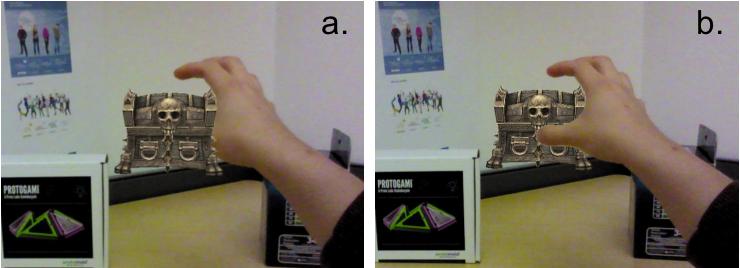
\includegraphics[width=246.666px, height=89.333px]{_image_occlusion-example}
\caption{a) Incorrect occlusion, b) correct occlusion \cite{du2016edge}.}
\label{fig:_image_occlusion-example}
\end{figure}

As mentioned earlier ``occlusion handling'' in AR is the name of functions that tries to solve the problem of occlusion between virtual content and real objects. I.e. if real objects are closer in distance to the user than the virtual objects, these objects are supposed to be fully or partially occluded (see fig. \ref{fig:_image_occlusion-example}) . If not, the user may lose their perception, making it harder to sense distances, size and depth of the virtual content \cite{shah2012occlusion}.

Researchers at European Computer-industry Research Centre (ECRC) introduced a taxonomy for these functions, categorizing them into model-based methods and depth-based methods \cite{breen1996interactive}. Both of these methods tries to solve the occlusion problem but in different ways and they each have their own strengths and weaknesses. The challenge that these methods face is to, in real-time, construct the geometric model of the occluding real objects and estimate the pose and position of the constructed objects as close as possible to the actual real objects \cite{fortin2006handling}. Then the actual occlusion effect will be fairly simple to achieve and similar for both methods. Both of them use some sort of Z-buffering technique, meaning that pixels of the virtual content that should be occluded are pushed down the depth buffer by the information retrieved about the surrounding environment.

The model-based method involves all occlusion handlers that need a 3D model representation of the surrounding environment to function. This model can either be manually created \cite{breen1996interactive, fuhrmann1999occlusion}, defined by the user \cite{ong1998resolving, lepetit2000semi, tian2010real} or retrieved by depth sensors \cite{tian2015handling}. Breen et al. \cite{breen1996interactive} performed one of the first model-based attempts for occlusion in AR by manually creating models of real objects in the current environment. They found the occlusion to be accurate but they also concluded that manually creating detailed models of complex scene is ``difficult or impossible''. Fuhrmann et al. \cite{fuhrmann1999occlusion} tried to achieve accurate occlusion in a collaborative AR setting, which meant that static objects like furniture, dynamic objects like tools as well as the human body needed to be included in their occlusion handler. They achieved this by pre modelling so called ``phantoms'' of all types of objects, and then aligning them with the corresponding real objects using magnetic trackers. \cite{ong1998resolving, lepetit2000semi} created a semi-automatic method where the user had to trace the silhouette of occluding objects and then their function defined a 3D model out of the traced data.  Tian et al. \cite{tian2010real} had a similar approach by letting the user trace the occluding objects, but the trace information was used for object tracking instead of conversion into a 3D model. Tian et al. \cite{tian2015handling} used a RGB-D camera to first construct a 3D model of the environment in an offline stage and then they mapped this 3D model to the depth information retrieved in an online stage. By doing this they achieved a real-time solution that accepted an arbitrary position and orientation of the camera. However it required a static environment and they also concluded that prefetching the 3D model of the environment in an offline stage is not ideal. 

Depth based methods include the functions that withdraw depth information of the surrounding environment in real-time. This depth information, or depth map, can then be converted into a 3D model of the environment used for the occlusion effect \cite{breen1996interactive} or the depth information can be applied straight away to the Z-buffer in each rendering cycle \cite{wloka1995resolving}. Compared to the model-based method, this method do not require any previous information about the environment \cite{shah2012occlusion}. The depth map can be retrieved by using a stereo camera \cite{breen1996interactive, wloka1995resolving, schmidt2002dense, zhu2010handling}, RGB-D cameras \cite{du2016edge}, Time-of-Flight (TOF) cameras \cite{fischer2007using}, and LADAR technology \cite{behzadan2010scalable}. Wloka et al. \cite{wloka1995resolving} conducted one of the earliest attempts of resolving occlusion in AR systems using a depth-based method with a stereo camera setup. They achieved the creation of the first real-time depth-based occlusion handler for AR, and the retrieved depth information was used for Z-buffering in order to create the occlusion effect. However, they found their algorithm to have difficulties in calculating depth on ``rectangular image areas that are evenly lit, non-textured and horizontal''. Breen et al. \cite{breen1996interactive} was also early in research for occlusion in AR but compared to Wloka et al. \cite{wloka1995resolving} they used the depth map to construct a 3D model of the surrounding environment. They found that 3D reconstruction was time consuming since the model became invalid as soon as the camera changed position or orientation. More recent depth-based attempts using a stereo camera include \cite{schmidt2002dense} who achieved pixel perfect occlusion almost in real-time by creating dense disparity maps. Zhu et al. \cite{zhu2010handling} fused the depth information from a stereo camera with color and neighboring pixels information. Their fusion algorithm achieved an accurate and robust result since when either the depth, color or neighboring pixel information was poor they could complement each other. Du et al. \cite{du2016edge} introduced an ``Edge Snapping-Based'' depth enhancement to reduce the noise retrieved from RGB-D cameras that are used for occlusion in AR. By adding edge tracking algorithms they enhanced the occlusion effect significantly compared to using only the raw depth data. Fischer et al. \cite{fischer2007using} combined a regular color camera with a TOF camera to retrieve depth information of the environment, but they struggled with noise from the TOF camera as well as synchronizing both the color camera and the TOF camera. Behzadan et al. \cite{behzadan2010scalable} achieved an occlusion handler that was functioning in a dynamic AR environment, both outdoors and indoors, in real-time. However, their setup included a heavy and expensive LADAR camera that the user carried on their back.

The model-based method has an advantage in not needing special hardware or big computing power when the application is running, however depth sensors can be used when retrieving the 3D model of the environment \cite{tian2015handling}. The method's obvious disadvantage is that the model of the environment needs to be acquired before hand \cite{breen1996interactive, shah2012occlusion}, making it only usable for predefined static environments. It may also be difficult to create detailed models of complex environments. However when the model is acquired the model-based method has proven to be robust and not having any visual artefacts, given that the model perfectly aligns with the real objects \cite{breen1996interactive}.

The advantages of the depth-based method is that it does not require a predefined 3D model, making it possible for usage in a dynamic and complex environment \cite{breen1996interactive, shah2012occlusion}. However, it has been proven to be time consuming \cite{tian2015handling} and that is not ideal that the depth map becomes invalid when the device changes position or orientation \cite{breen1996interactive, shah2012occlusion}. Depth sensing devices also produce a lot of noise, which create visual artefacts such as aliasing \cite{wloka1995resolving, shah2012occlusion, zhu2010handling}. Common for all the previous depth-based attempts is that they require certain conditions, special hardware and/or big computing power. Neither of them can be implemented on regular non depth-sensing devices that the users have today. This might change soon as depth sensing devices such as Google Tango and Microsoft Hololens is already available for consumers \cite{vergeTango, vergeHololens}.

Kasapakis et al. \cite{kasapakis2015determining} proposed an alternative approach to reconstruct the geometric model of the current environment, that did not require any special hardware or a predefined environment. However, it was not used for simulating an occlusion effect. They called their solution ``Geolocative Raycasting'' which determined the user's field of view (FOV) in an urban AR environment. By first querying geospatial data from \textit{OpenStreetMap} (OSM) and then using ray casting from the user's current geographical position (defined by a smartphone's GPS) onto the surrounding buildings (defined by their corresponding geospatial data from OSM), they could in real-time create a polygon representing the area the user currently could see (see fig. \ref{fig:_image_kasapakis}). The area that was withdrawn from the ray casting function was then used to determine if the user could or could not see a Point-of-Interest (POI), by marking it with a red color. The results were a stable and accurate function, and they concluded that geospatial data can be used to construct the model of the surrounding environment. However, Kasapakis et al. \cite{kasapakis2015determining} only used geospatial data to determine the user's FOV in 2D (latitude and longitude). It is also important to note that in their function only included buildings, other objects such as trees, cars or people did not affect the detection of if the POIs were visible or not.
\begin{figure}
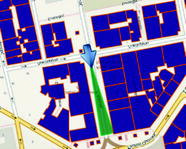
\includegraphics{_image_kasapakis}
\caption{Visualization of the ``Geolocation Raycasting'' technique used for determining the user's current FOV \cite{kasapakis2015determining}.}
\label{fig:_image_kasapakis}
\end{figure}

\subsection{Motivation and research question}
Previous studies have tried to create pixel-perfect occlusion for AR systems, but they have all required either special hardware or a predefined static environment. This study has tried to do the opposite. It proposes a new dynamic occlusion handling for outdoor AR systems, functioning on regular smartphones without depth sensing capabilities and in a dynamic outdoor urban environment. However, the proposed solution do not try to achieve pixel-perfect occlusion. It tries to create an occlusion effect that is efficient enough, i.e. it tries to give users an acceptable sense of perception and depth. Also will it not include all real world objects in the occlusion function, it will only include buildings. The study continues the work of Kasapakis et al. \cite{kasapakis2015determining} by using geospatial data from OSM in AR. But compared to Kasapakis et al., the solution in this study converts geospatial data of buildings from OSM into 3D models, allowing virtual AR 3D models to be occluded by real world buildings.  

The research question of the study, and the motivation for developing the proposed solution, were:
\begin{quote}
What are the results of occluding virtual 3D objects by real world buildings using geospatial data in an outdoor urban Augmented Reality environment?
\end{quote}

\subsection{Concepts and technologies}
\subsubsection{Tracking techniques}
Tracking is the technologic term for how the AR device's pose and field of view is estimated in relation to the real world \cite{zhou2008trends}. AR is often divided into three categories based on the type of tracking technology being used \cite{zhou2008trends}. The first category is \textit{vision-based tracking}, which uses computer vision on the video stream from the camera on the device to estimate its pose in relation to real world objects \cite{zhou2008trends}. The first vision-based tracking methods were tracking markers such as QR-codes. Then came tracking of images and the environment with 3D models, and finally \textit{SLAM} which estimates the pose and position of the device where no model of the environment is available \cite{azuma2016most}. The second category is called \textit{sensor-based tracking} which uses magnetic, acoustic, inertial, optical and/or mechanical sensors to determine the device's pose and FOV \cite{zhou2008trends}. In mobile AR these sensors are often GPS, magnetometer and gyroscope \cite{zhou2008trends}. Sensor-based tracking is more suitable for outdoor AR since it does not require any type of marker tracking which makes it more versatile \cite{cirulis20133d}. However, sensor-based tracking for mobile AR has issues with inaccuracy of the sensor which introduces noise to the device pose estimation function \cite{cirulis20133d}. The third and last category is called \textit{hybrid-based tracking} which is a combination of the two previous \cite{zhou2008trends}. 

\subsubsection{Geospatial data and OpenStreetMap}
Geospatial data is data regarding the Earth's features \cite{ogcFaq}. One provider of open geospatial data is the crowd-sourced initiative \textit{OpenStreetMap} (OSM) \cite{osmAbout} and their data can be retrieved through their API, called \textit{Overpass API} \cite{osmOverpass}.

\subsubsection{Argon.js}
Argon.js is a \textit{Software Development Kit} (SDK) for AR created by MacIntyre et al. \cite{macintyre2011argon}. The purpose of the SDK is to give developers a tool to create applications using common web technologies such as WebGL, HTML, CSS and Javascript with support of vision-based and sensor-based tracking. It is accompanied with the Argon browser, which is a native mobile web browser application with support for AR developed with Argon.js. The Argon browser was created due to the problem where different earlier AR all had their own mobile application, making it impossible to use several of them in parallel on the same device. The Argon browser creates a common ecosystem for different kinds of AR making it possible to use them simultaneously and thereby solving this problem \cite{macintyre2011argon}. 

\section{Method}
For the purpose of this study an experimental AR application was developed using sensor-based tracking. The application visualized a future building, that had not been built, in Stockholm, Sweden. The application included the developed model-based occlusion handler, and the models were created from geospatial data of buildings from OSM. A model-based approach was used since it should function on devices without depth sensors. 

The final goals for the proposed occlusion handler were:
\begin{itemize}
\item Converting geospatial data of buildings from OpenStreetMap (OSM) to 3D models.
\item Use the models from the conversion to create a model-based occlusion handler of buildings in a dynamic outdoor urban AR environment.
\item Functioning on regular non depth-sensing smartphones equipped with a camera, Internet connection, GPS, gyroscope and magnetometer.
\item The goals above will be achieved on the cost of not creating pixel-perfect occlusion.
\end{itemize}

This application was evaluated with a performance test and a user test. The performance test included execution time measurements of the creation of 3D models out of the geospatial response from Overpass API. The execution time for updating the position of the occlusion models for each render frame were also measured. Lastly a frame rate (FPS) analysis was made to see if the proposed occlusion handler affected the overall performance on the WebGL scene by comparing it to usage without the occlusion handler activated.

A user study were then conducted with 13 participants in the ages 22-31. They were instructed to use the developed AR application freely, first with the occlusion handler deactivated and then activated. However, before the test started they were given information about the purpose of the study in order to know what to evaluate. After using the prototype they were given a questionnaire consisting of 13 statements with Likert scale \cite{likert1932technique} type of options ranging from ``Strongly disagree'' to ``Strongly agree''. The answers were then scored in the analysis from 1 to 5 with 1 equal to ``Strongly disagree'' and 5 equal to ``Strongly agree''. The purpose of the user study was to evaluate if the develop occlusion handler was efficient enough to give the users a sense of perception and depth, i.e. did the occlusion handler reach the goal of occlusion handlers. 

The proposed occlusion handling function was not evaluated with a root-mean-square error or similar. This decision was made because pixel-perfect occlusion were never a goal of the developed solution. Instead the visual effect of the occlusion handler, i.e. how it looked on the screen on the device, is presented with screenshots.

All tests were conducted on an Apple iPhone 5S with 1 GB RAM, Dual-core 1.3 GHz Cyclone CPU and PowerVR G6430 GPU.

\section{Result}
This section covers the result of this study. It starts off by listing the technologies used in the study's experimental application. After that, a description of the algorithm used for the occlusion handler will be presented. Finally are the results of the occlusion handler presented in three different topics, first the occlusion result (i.e. the visual effect of the occlusion handler), then the performance test and last the result from the user study.

\subsection{Application structure}
The entire application was developed to be used within the Argon browser app, so the AR features (the sensor-based tracking) was made with the Argon.js SDK. Since the application was made for the Argon browser, the application was developed using web technologies, i.e. WebGL, HTML and JavaScript. Three.js, a 3D computer graphics library for WebGL \cite{threeAbout}, was used for the 3D rendering.

\subsection{Occlusion algorithm}
Step one in the algorithm of the occlusion handler is to query geospatial data of buildings from Overpass API. The query is made in the Overpass query language called \textit{Overpass QL} (see listing ~\ref{lst:overpass_query}). Before querying the API, the algorithm needs a radius \textit{r} and geolocation \textit{L} as input. \textit{r} and \textit{L} determines a bounding circle on the earth's surface with \textit{r} as the circle's radius and \textit{L} as the circle's center. All buildings within this bounding circle will be fetched from Overpass API.

\begin{lstlisting}[caption={Example query to Overpass API, given in Overpass QL, with r set to 100 and L set to (59.329553,18.079065).}, label={lst:overpass_query}]
[out:json];
(
  way["building"](around:100,59.329553,18.079065);
  relation["building"](around:100,59.329553,18.079065);
);
out body;>;out skel qt;
\end{lstlisting}

The response from Overpass API with geospatial data of the buildings is then encoded in the \textit{OSM JSON} format (see listing ~\ref{lst:overpass_response}).

\begin{lstlisting}[caption={Example response from Overpass API of the National Museum of Fine Arts in Stockholm, Sweden, given in OSM JSON.}, label={lst:overpass_response}]
{
  "type": "way",
  "id": 24968329,
  "nodes": [
    1406078451,
    1863238948,
    2554104722,
    ...
  ],
  "tags": {
    "building": "museum",
    "building:colour": "brown",
    "building:levels": "3",
    "description": "Sweden's leading museum for art and design.",
    "name": "Nationalmuseum",
    "name:en": "National Museum of Fine Arts",
    "opening_hours": "Tu-We, Fr-Su 10:00-17:00; Th 10:00-20:00",
    "roof:colour": "MediumAquamarine",
    "source": "yahoo_imagery",
    "tourism": "museum",
    "website": "http://www.nationalmuseum.se",
    "wheelchair": "yes",
    "wikipedia": "sv:Nationalmuseum"
  }
}
\end{lstlisting}

As seen in listing \ref{lst:overpass_response} a great variation of data is listed in the response from OSM. The algorithm in this study utilizes that each building has references to multiple so called \texttt{nodes} which are the data representing a geolocation (see listing \ref{lst:overpass_node}). In general, a node is a specific geolocation represented by a latitude and a longitude value. 

\begin{lstlisting}[caption={Node that is referenced by the National Museum of Fine Arts in Stockholm given in OSM JSON.}, label={lst:overpass_node}]
{
  "type": "node",
  "id": 1863238950,
  "lat": 59.3285374,
  "lon": 18.0785740
}
\end{lstlisting}

Nodes referenced by a building specifically represents the geolocation of a corner on the building.  The National Museum of Fine Arts has for example 34 node references, making the polygon seen in fig. \ref{fig:_image_nationalmuseum2d}.

\begin{figure}
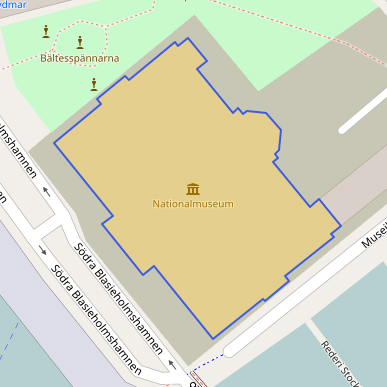
\includegraphics[height=200px, width=200px]{_image_nationalmuseum2d}
\caption{The nodes, or corners, from Overpass API making the ground floor polygon of the National Museum of Fine Arts in Stockholm.}
\label{fig:_image_nationalmuseum2d}
\end{figure}

The next step in the algorithm is to transform the OSM JSON data to \textit{GeoJSON} \cite{geojson}. GeoJSON is an alternate format to OSM JSON that makes it easier to traverse and extract desired data in the next steps of the algorithm. This step is not necessary for the occlusion handler to function, but it was included to make the development of the next steps easier.

As mentioned earlier, the occlusion handler uses a model-based method, therefore is the next step to create 3D models out of the geospatial data fetched in previous steps. As seen in fig. \ref{fig:_image_nationalmuseum2d}, the nodes referenced by each building creates a polygon representing the ground floor. The next step in the algorithm is to elevate this polygon along the y-axis to create a 3D model (see fig.  \ref{fig:_image_nationalmuseum3d}). The height of this elevation is defined by the \texttt{building:levels} tag, representing how many levels the building has, that is included in the Overpass API result (see listing \ref{lst:overpass_response}). The level amount are then multiplied by 3 to decide the height in meters. Also, if the building has a \texttt{roof:shape} (not included in listing \ref{lst:overpass_response}) tag that is not equal to \texttt{flat}, meaning that the real building has a roof that is not flat, the level amount is increased with one unit. However, since OSM do not have level data for all buildings the algorithm falls back and sets the levels to the integer 3, i.e. three is the default number of levels in the algorithm. The creation of the model mesh is done by using the \textit{ExtrudeGeometry} function in Three.js \cite{threejsExtrudegeometry}. 

\begin{figure}
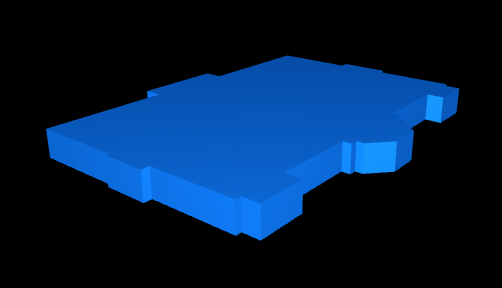
\includegraphics[width=245px, height=147px]{_image_nationalmuseum3d}
\caption{3D model of the National Museum of Fine Arts in Stockholm created by using geospatial data from OSM.}
\label{fig:_image_nationalmuseum3d}
\end{figure}

Before creating the models the algorithm waits until the device has initialized its GPS and the Argon.js environment has retrieved the geolocation of the device. All previous steps is done upon launch of the application. The algorithm awaits the geographical position of the device to be initialized before creating the models because this makes the rotation of the created models accurate and aligned with the real world buildings. The reason for this is that Argon.js always positions the device in origo in the WebGL scene.

The next step is to, in each render loop, accurately position the created occlusion models in the Argon.js environment in respect to the device so it aligns with their corresponding real buildings. Since the application uses sensor-based tracking, each building are positioned at the same geographical position as the first node (corner) that the building is referencing in its geospatial data. Each building also has its local origo around this node and, as mentioned earlier, it is already correctly rotated resulting in the entire model aligning with its real building.

The last step of the algorithm is to make all the occlusion models transparent and use them for Z-buffering, just like many previous attempts. This was made by setting the \texttt{colorWrite} property on the Three.js \textit{Material} object to false, and setting the \texttt{renderOrder} on the Three.js \textit{Mesh} object of the occlusion models to an integer value lower than the virtual building \cite{threeMaterial, threeMesh}.

The source code of the proposed solution is available at: \url{https://github.com/johankasperi/argon-osm-occlusion}

\subsection{Visual effect}

\begin{figure*}
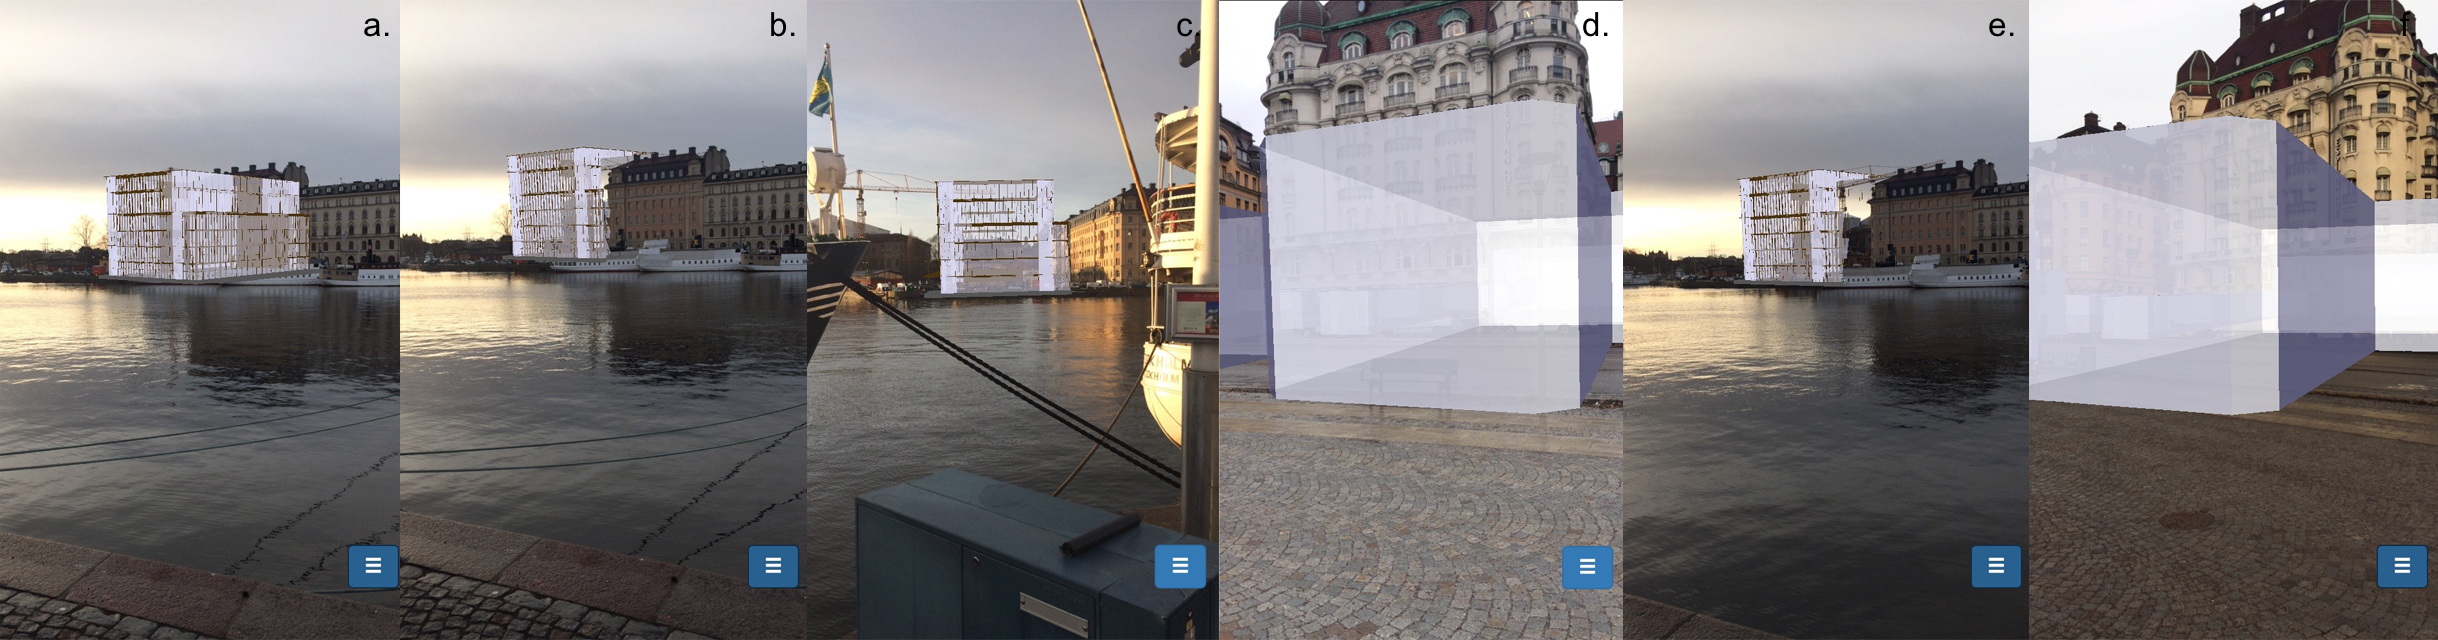
\includegraphics[width=490px, height=129px]{_image_visual-effect}
\caption{Visual effect of the developed occlusion handler. a) Occlusion deactivated. b) Occlusion activated. c) Occlusion activated but no real buildings in line-of-sight. d) Occlusion 3D model aligned with real world building. e) Occlusion activated but position of virtual building incorrect. f) Occlusion 3D model not aligned with real building}
\label{fig:_image_visual-effect}
\end{figure*}

The visual effect of the developed occlusion handler can be seen in fig. \ref{fig:_image_visual-effect}. Fig. \ref{fig:_image_visual-effect}a shows how the virtual building in the application looked when the occlusion handler was deactivated. The building appears in front of a real building even though this building is supposed to be in the line-of-sight between the user and the virtual building. Compare this to fig. \ref{fig:_image_visual-effect}b where the occlusion handler is activated, the virtual building's vertices is pushed down the depth buffer by the transparent occlusion models, resulting in the virtual building being occluded along the edge of the building that is in the line-of-sight.  Fig. \ref{fig:_image_visual-effect}c shows the visual effect when the occlusion handler is activated but there is no real building in the line-of-sight, resulting in no occlusion on the virtual building.

Fig. \ref{fig:_image_visual-effect}d shows a opaque occlusion model of a building in Stockholm, Sweden. The occlusion model aligns well with its real building, but as you can see the occlusion model is not as detailed as its building. Fig. \ref{fig:_image_visual-effect}d also shows that the height of the occlusion model does not match the real building. This particular building did not have any level data stored by OSM, making the occlusion algorithm fallback to creating the model with a height of 9 meters. Also occlusion models for buildings with level data stored by OSM did not match the height of their real buildings sometimes. Causes of this was the algorithms general assumption that one level equaled 3 meters and that the height of the roof was not included in the OSM data.

The application used a sensor-based tracking method, relying on sensor such as GPS, gyroscope and magnetometer to position the virtual content in the real world. Fig. \ref{fig:_image_visual-effect}e and fig. \ref{fig:_image_visual-effect}f shows the issues emerging using a sensor-based method. The sensors of the device in this study was from time to time inaccurate, which resulted in the virtual building as well as the occlusion models being positioned wrong. For example, fig. \ref{fig:_image_visual-effect}e shows the virtual building being occluded by the occlusion model, but since both the virtual building and the occlusion models has incorrect positions due to the sensors, the edge of the occlusion does not align with the real building at all.

\subsection{Performance}
All of the performance tests were conducted with four different input sets. Each set had a different bounding circle radius (\textit{r}) as input parameters to the algorithm. These different radiuses retrieved different amount of buildings from the Overpass API due to the larger area of buildings to be included, resulting in different impact on the performance of the algorithm. The geolocation of the circle (\textit{L}) were always set to a position in central Stockholm, Sweden (see tab. \ref{tab:input_sets}).

\begin{table}
  \caption{Radius (r) and location (L) input parameters to the occlusion algorithm and retrieved amount of buildings used for all of the performance tests}
  \label{tab:input_sets}
  \begin{tabular}{lllr}
    \toprule
    Input set & Radius (\textit{r}) & Location (\textit{L}) & \# Buildings\\
    \midrule
    1 & 100 m & 59.3474572, 18.0737809 & 6\\
    2 & 200 m & 59.3474572, 18.0737809 & 35\\
    3 & 500 m & 59.3474572, 18.0737809 & 159\\
    4 & 1000 m & 59.3474572, 18.0737809 & 439\\
    \bottomrule
  \end{tabular}
\end{table}

The first performance test was the average execution time measurement for creating the occlusion 3D models out of the geospatial data from Overpass API (see fig. \ref{fig:_image_performance-create-models}). The algorithm ran for 100 iterations for each input set. The 100 iterations made the sample size for measuring the average execution time for each input set. This sample size made the result 95 \% confident (using a t-distribution) and the confidence interval magnitude about 10 \% of the average execution time for each input set (see fig. \ref{fig:_image_performance-create-models}). For example, the confidence interval for input set 1 were 1.25 ms. The results show that as the number of buildings included in the algorithm increases, the execution time for creating all of the occlusion models increases (see fig. \ref{fig:_image_performance-create-models}). 

\begin{figure}
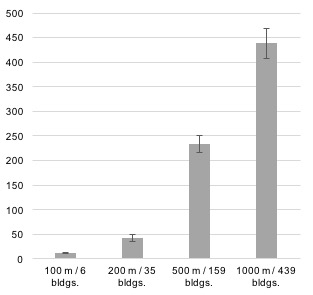
\includegraphics[width=200px, height=188px]{_image_performance-create-models}
\caption{Average execution time (ms) for creating models out of geospatial data for the four different input sets to the algorithm.}
\label{fig:_image_performance-create-models}
\end{figure}

The average execution time for updating the position of the occlusion models in each render loop, due to update of the device position or orientation are presented in fig. \ref{fig:_image_performance-rendertime}. This average was measured during 5 minutes of regular usage of the prototype for each input set (see tab. \ref{tab:input_sets}). The results show that as the number of real world buildings included in the occlusion increases, the average execution time for updating all of the occlusion models also increases (see fig. \ref{fig:_image_performance-rendertime}).

\begin{figure}
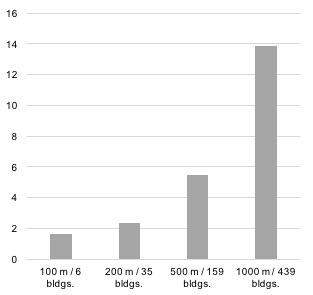
\includegraphics[width=200px, height=188px]{_image_performance-rendertime}
\caption{Average execution time (ms) for updating the position of the occlusion models in each render loop.}
\label{fig:_image_performance-rendertime}
\end{figure}

The last performance test conducted were the FPS analysis. This test were also measured during 5 minutes of regular usage of the app for each input set. However, this test were first conducted with the occlusion handling function deactivated to get an comparison value. The results show that the occlusion handling function had no impact on the prototype's FPS, no matter how many real world buildings that were included in the occlusion. The average FPS was 30 for input set 1-5 as well as for when the occlusion handling was deactivated.

\subsection{User study}

The 13 participants in the user study had an average age of 27.3 and median of 27. 10 of them were engineering students and the other 3 had non-engineering jobs. 6 of the participants answered ``Strongly agree'' or ``Agree'', 4 ``Neutral'' and 3 ``Strongly disagree'' or ``Disagree'' when asked if they have a lot experience from AR. The average on this statement was 3.23 and median 3. When asked if they had any experience from AR and occlusion handling neither answered ``Strongly agree'' or ``agree'', 3 answered ``neutral'' and the rest answered ``Strongly disagree'' or ``Disagree''. This statement got an average of 2.38 and median of 2. The participants were then asked about their previous knowledge about the future building visualized in the prototype, and its placement in Stockholm. 3 participants agreed that they had knowledge about the position of this building but the majority strongly disagreed to this statement. The average on this statement was 2.15 and median 2.

The participants were then given a statement about the prototype in general, not focusing on the occlusion handling function. On the statement ``My general impression of the prototype was good'' 10 of the participants answered ``Strongly agree'' or ``Agree'', 2 answered ``Neutral'' and 1 ``Disagree''. This resulted in an average of 3.85 and median of 4. 

The last statement before the statements about the occlusion handler were about the tracking. Since the sensor-based tracking had proved to be inaccurate sometimes the participants were asked if the tracking affected their experience of the application. The majority answered ``Agree'' on this statement (see fig. \ref{fig:_image_user-licert}) and the average was 3.15 and median 4.

\begin{figure*}
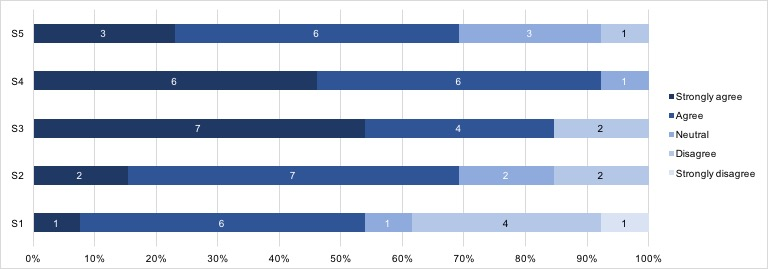
\includegraphics[width=490px]{_image_user-licert}
\caption{Answers from statements 1-5. Statement 1: ``The tracking affected my experience of the prototype''. Statement 2: ``The occlusion handling in this prototype was satisfying''. Statement 3: ``The prototype was better with the occlusion handling activated compared to having it deactivated''. Statement 4: ``The occlusion handling in this prototype gave me a better depth perception''. Statement 5: ``The occlusion handling in this prototype gave me an experience that the virtual content was mixed/interacted with the real buildings''.}
\label{fig:_image_user-licert}
\end{figure*}

On the statement ``Occlusion handling is important in applications with location based Augmented Reality'' a majority of the participants answered ``Agree'' or ``Strongly agree''. When asked if the occlusion handling in this prototype was satisfying, the majority agreed to this statement (see fig.  \ref{fig:_image_user-licert}) and the statement got an average of 3.69 and median of 4.

Most of the participants answered that they agreed that the prototype was better when the occlusion handler was activated compared to having it deactivated (see fig. \ref{fig:_image_user-licert}). This statement got an average of 4.23 and median of 5. 

The next topic in the user study regarded depth perception, one of the main goals for occlusion handling functions in AR. All participants except one agreed or strongly agreed that they got a better depth perception due to the occlusion handling function (see fig. \ref{fig:_image_user-licert}), giving it an average of 4.38 and median of 4. They were also asked if they got a better depth perception with the occlusion handling activated compared to having it deactivated. 13 of the participants agreed to this statement, giving it an average of 4.54 and median of 5.

The last topic of the user study concerned the users experience of whether the virtual building was more mixed and interactive with the real buildings or not, which was another main goal for occlusion handlers. The participants were asked to answer the statement ``The occlusion handling in this prototype gave me an experience that the virtual content was mixed/interacted with the real buildings'' and a majority of the participants agreed to this (see fig. \ref{fig:_image_user-licert}). The average was 3.85 and mean 4. They also answered the statement ``The occlusion handling in this prototype gave me a better experience that the virtual content was mixed/interacted with the real buildings compared to having it deactivated'', in order to compare this topic to when they had the occlusion handler deactivated. 9 participants agreed and 4 participants strongly agreed to this statement, resulting in an average of 4.31 and median of 4.

\section{Discussion}
In this section the results of the study will be discussed and analyzed in order to answer the research question. The results are also  compared with previous similar attempts and the section finishes with proposing further research within the area. 
The purpose of this study was to develop and evaluate a dynamic occlusion handling function for outdoor urban AR that did not require any special hardware more than a smartphone or a predefined static environment. These goals would be reached on the cost of not achieving pixel perfect occlusion and that only real world buildings would be included. 

The evaluation of the developed occlusion handler would then answer the research question:
\begin{quote}
What are the results of occluding virtual 3D objects by real world buildings using geospatial data in an outdoor urban Augmented Reality environment?
\end{quote}

Looking at the visual effect result (see fig. \ref{fig:_image_visual-effect}b) one can see that the virtual building are occluded along the roof and corner of the real world building. The same results were achieved from several different angles with different buildings in the line of sight between the device and the virtual building. Also the virtual building were fully visible when there was no real building in the line of sight (see fig. 5c), and not visible at all when the entire virtual building was behind a real building. Given these results the study's occlusion handler is functioning as expected, it simulates the effect of how it would have been if the virtual building was a real building placed at the same location. However, it produces some visual artefacts, for example the occlusion of the virtual building does not align with the edge of the real building perfectly. This means that the proposed solution is not handling occlusion in AR realistically. But the goal of the proposed solution was never to create pixel-perfect occlusion, it was to create an occlusion handler that was efficient enough. Meaning that it would fulfill the goals of occlusion handlers, to give the users a sense of depth, size and distance and the feeling that the virtual and real objects was mixed and interacted \cite{shah2012occlusion}. Looking at the answers from the user study of the questions regarding this it might seem so. 12 of 13 participants in the user study thought that their depth perception got better (see fig. \ref{fig:_image_user-licert} and \ref{fig:_image_user-licert}) agreed that the virtual content felt more mixed with the real buildings (see fig. \ref{fig:_image_user-licert}) when trying the prototype. But further user studies with more participants from a more heterogenous selection group is needed to confirm if the proposed occlusion handling function reached the goals of occlusion handlers.

The method used for occlusion handling in this study had two main issues, which also caused the visual artefacts. The first issue was that the geospatial data from OSM could not be transformed to detailed occlusion models. One of these details missing are those regarding the roof of the real world building. Looking at fig.  \ref{fig:_image_visual-effect}d you can see that the roof of the occlusion model is completely flat, which was the case with all occlusion models. Obviously real world buildings have much more detailed roofs with slants, chimneys etc. OSM has data about these type of details for some buildings \cite{osm3Dbuildings} that was not implemented in the solution of this study. The main reason for this was that few buildings in Stockholm had any roof shape data and that this data is not a reflection of the reality. However, future studies could explore using the roof shape data from OSM. Compared to the roof, the occlusion behind corners and walls of real buildings was better. The cause for this was that data of the nodes, or corners, from OSM was more accurate and aligned with the corners of the real buildings.

Another detail that was missing in the geospatial data was an accurate height of the real buildings. The \texttt{building:levels} data, that was used for setting the height of the occlusion models, was missing on a majority of the real buildings tested in this study. So for all of these buildings the algorithm used the default level amount (see 4.2). This resulted in that all of the occlusion models for buildings that lacked level data had a height mismatch to their real building. Also, using the arbitrary height of 3 meters per level also caused a height mismatch since the height per level for a building is fairly unique. 

Since the building height and roof details was troublesome and the building corners and walls were accurate the proposed solution could be altered when taking these findings into consideration. This alternative algorithm could create the occlusion models with infinite height instead of trying to match the height with the real buildings. Obviously would all virtual content positioned above buildings be occluded, but that alternative might be better than trying to incorrectly, due to incorrect height or roof data, occlude virtual content along the roof of the real buildings. This alternative would utilize the strength of the current state of the OSM database, the nodes or corners, and skip the weaknesses, the building height and roof details. 

The second issue of the prototype causing a lot of the visual artefacts was the tracking method. As mentioned earlier, the prototype used sensor-based tracking for placing the virtual content in the real world. The results show that this was a mistake, a lot of the time were the virtual building and the occlusion models incorrectly positioned (see fig \ref{fig:_image_visual-effect}e and \ref{fig:_image_visual-effect}f). Previous studies has proven that it is important for the occlusion models to align with the real objects and since the tracking in this study struggled with that, all results have been affected. For example, the occlusion of the building in fig. \ref{fig:_image_visual-effect}b might align with the edge of the building better if the positioning of the content was more precise. This issue was also confirmed by the user study, 7 participants answered that the sensor-based tracking affected their experience (see fig. \ref{fig:_image_user-licert}). Even though this study was not focusing on or evaluating any tracking technology it is obvious that an alternative tracking technology should have been used.

Comparing the proposed solution to previous studies the visual effects have some differences. All previous studies have tried to achieve pixel-perfect occlusion, with either a depth- or model-based method, and many of them have somewhat succeeded. But all of these have required either special hardware or a predefined static environment, making it impossible to easily implement on AR applications for smartphones. As mentioned earlier, this study has done the opposite. The visual effect of the occlusion is far from perfect, but it can be implemented on a regular non depth-sensing smartphone. The results show that the main goal of an occlusion handler does not need pixel-perfect occlusion. It could instead be simplicity. Even though it had some errors, the occlusion handler was appreciated by the participants of the user study (see fig. \ref{fig:_image_user-licert} and \ref{fig:_image_user-licert}) and as mentioned earlier it could achieve the ultimate occlusion handler goals. Also the visual artefacts due to poor occlusion models could be compared with the depth sensing noise experienced in previous studies. The proposed solution was also light in computation, the impact on the frame rate of the WebGL renderer was insignificant and instantiating all the occlusion models upon application launch were fast (see fig. \ref{fig:_image_performance-create-models}). Even though it is difficult to compare the computation power needed for the proposed solution to previous studies, since previous studies has been more advanced, this at least means that the solution's negative aspect of simulating occlusion poorly is countered with being lightweight. But it is important to note that the proposed solution only included buildings in the occlusion. Previous studies, especially the depth-based, have included all arbitrary objects in the current AR environment. This was also mentioned by the participants of the user study, several of them asked if the virtual building was occluded behind cars, signs and similar.

As mentioned in the theory section, the challenge for occlusion handlers is to  construct the geometric model of the occluding real objects in real-time as well as estimate the pose and position of the constructed objects as close as possible to the actual real objects. The same challenge exists for all type of functions that tries to simulate any physical interaction between the real objects and the virtual content, such as shadowing or collisions. It needs to know the state and form of the current environment. This is also what the solution in this study does, it uses geospatial data to recreate the models of the buildings in the current environment. This means that it is possible to use the same approach for all the other physical simulations.

That the results show that using geospatial data, without perfect reconstruction of the environment, can create efficient enough physical simulations is positive for the future development of AR. Mainly because smartphones are currently the main driver for making AR available for everybody, making it important to find alternate methods that can run on them. The approach of using geospatial data could be one of these alternatives. However, all these results might only be applicable until AR hardware such as Microsoft Hololens and Google Tango has taken over a larger part of the market. Both of them, and probably many not yet invented AR devices, are equipped with depth sensors. And since depth sensors constructs the current environment in real-time very accurately, all of the alternative methods for non depth sensing devices might become obsolete. But until then this study shows that geospatial data could play a role in making the AR field closer to its ultimate goal: 

\begin{quote}
\textit{``The ultimate goal will be to generate virtual objects that are so realistic that they are virtually indistinguishable from the real environment''} \cite{azuma1997survey}
\end{quote} 

However, due to methodological reasons, some of the conclusions in this study cannot be confirmed. The two main issues, that have been described above, are the selection of tracking method and the selection group of the user study participants. If a more accurate tracking method would have been used the results might have been different, since previous studies have confirmed the importance of perfect alignment of the occlusion models. The background of the user study participants also makes it difficult to confirm if the proposed solution reaches the goal for occlusion handlers. A majority of them had previous AR experience (see 4.5) and had a computer science background, so they probably had more knowledge about the challenges and implications of the AR medium in general. Different results may have been gathered if the user study's selection group was more heterogenous.

Future studies within the area of this study should first of all try  to fix the issues with the method described above in order to confirm the conclusions. First, this means using the same geospatial approach but with an alternative tracking method. Probably a hybrid-based tracking method which utilize the strengths of the smartphone's sensors and the vision through its camera. Secondly, further studies should also conduct a more thorough user study with more participants with more diverse backgrounds. There are also some improvements that could be made to the proposed occlusion algorithm which invites for interesting future studies. One of them is to include the roof shape data from OSM in order to create more detailed occlusion models. Another is to alter the algorithm to create occlusion models with infinite height, which as described earlier utilizes the strength of the current state of the OSM database. Other interesting future studies could be to use the same geospatial approach but for other physical simulations, for example shadowing or collisions, and see if similar conclusions as in this study can be drawn. Lastly it would be interesting to explore using different types of geospatial data, from perhaps other sources, to be able to one day fully reconstruct the current environment of all real objects in the scene with the geospatial data approach. 

\section{Conclusion}
This study has explored using geospatial data to construct the geometric model of buildings in a dynamic outdoor environment. This model have been used to simulate occlusion between virtual content and real buildings in AR. The goal has been to create and evaluate a simple but yet efficient enough occlusion effect that can run on a regular smartphone in any outdoor environment. The conclusions are that occlusion handlers using geospatial data can be efficient enough, since the function made the virtual content partially or fully occluded when a real building was in the line-of-sight. However, the study also shows that the geospatial data from OSM does not support creation of models that have the same level of details as the real buildings. For example features such as chimneys or slanted roofs was poorly represented by OSM and therefore not included in the occlusion. It was also found that the geospatial data from OSM does not provide accurate height data, if any, about the real buildings which resulted in a notable height differences between the occlusion models and the real buildings. 

The study has also shown that occlusion handlers for AR do not need to be pixel-perfect, which have been mostly researched in previous studies, to fulfill its ultimate goal. A majority of the participants in the conducted user study thought that their AR experience improved when the proposed solution was activated. This could mean that simpler methods to create the geometric model of the current AR environment could be used for mobile AR until depth-sensing devices gets more widely used. But any definite conclusions about this cannot be drawn due to issues with the sensor-based tracking. It produced a significant noise in the positioning of the occlusion models and the virtual content which affected the user experience.

\section{Acknowledgement}
I would like to thank my supervisor from KTH, Malin Picha Edwardsson, for the help and support while conducting this study. Also, thanks to Matilda E. Hanson, Thomas Hanusek and Blair MacIntyre for assisting me during the development stage of the prototype. Finally, a huge thanks to my partner in crime, Daniel Lindstr\"om.





\bibliographystyle{unsrt}
\bibliography{references}

\end{document}
